\section{Resultados}
%###########################
%########## AVG ############
\subsection{Dinámicas factorizables}
\begin{frame}{Dinámicas factorizables}
    Por dinámicas factorizables entendemos aquellas generadas por un hamlitoniano de la forma:
    \begin{equation}
        H=\nonumber
    \end{equation}
    Que se traducen en evoluciones unitarias de la forma:
    \begin{equation}
        H=\nonumber
    \end{equation}
    \begin{columns}
        \begin{column}{0.5\textwidth}
            El estado de máxima entropía es
        \end{column}
        \begin{column}{0.5\textwidth}
            La dinámica efectiva tiene expresión general
        \end{column}
    \end{columns}
\end{frame}

\begin{frame}{Partículas no interactuantes con diferente frecuencia de transición}
    \begin{columns}
        \begin{column}{0.5\textwidth}
            \begin{equation}
                \mcH=\sum_{k=1}^{n}\omega_{k}\pauli{3,k},\nonumber
            \end{equation}
            de tal forma que toda la evolución mantenga constante la componente en $\pauli{3}$. Explícitamente, las componentes del vector de Bloch del estado efectivo siguen las ecuaciones
            \begin{align}
                r_{1,\ef}(t)=&p_{1}r_{1,1}(t)-\sum_{k=2}^{n}p_{k}A_{k}\sin(2\omega_{k} t-\phi_{k})\nonumber\\
                r_{2,\ef}(t)=&p_{1}r_{2,1}(t)+\sum_{k=2}^{n}p_{k}A_{k}\sin(2\omega_{k} t+\theta_{k}),\nonumber
            \end{align}
            donde se omite la tercera componente, que no cambia, y
            \begin{align}
                A_{k}=\sqrt{r_{1,k}^{2}+r_{2,k}^{2}} & & \phi_{k}=\arccos\qty(\frac{r_{2,k}}{\sqrt{r_{1,k}^{2}+r_{2,k}^{2}}}) & & \theta_{k}=\arcsin\qty(\frac{r_{1,k}}{\sqrt{r_{1,k}^{2}+r_{2,k}^{2}}}).\nonumber
            \end{align}
        \end{column}
        \begin{column}{0.5\textwidth}
            El comportamiento de los términos de suma depende de las frecuencias $\omega_{k}$, pero la amplitud de estas funciones oscilatorias puede acercarse arbitrariamente a $\sum_{k=2}^{n} p_{k} A_{k}$. Esto no significa que el error explote. En realidad, como $0\leq A_{k}\leq 1\,\forall k$, entonces $0\leq\sum_{k=2}^{n} p_{k} A_{k}\leq 1$. 


Para obtener resultados más específicos, sea $p_{j}=p_{\text{np}}=\frac{1-p_{1}}{1-n}\,\forall\,j\neq 1$ y $r_{3,\ef}=0$. Por construcción del estado de máxima entropía compatible con $\rho_{\ef}$,
\begin{align}
    r_{k}=r_{\text{np}}=\tanh(p_{\text{np}} \lambda) & & r_{j,k}=r_{\text{np}}\frac{r_{j,\ef}}{r_{\ef}}.\nonumber
\end{align}
Esto significa que las expresiones previas se simplifican considerablemente, en efecto, las primeras dos componentes del vector pasan a ser
\begin{equation}\label{eq:}
    \begin{gathered}
        r_{1,\ef}(t)=p_{1}r_{1,1}(t)-p_{\text{np}}r_{\text{np}}\sum_{k=2}^{n}\sin(2\omega_{k} t-\phi)\\
        r_{2,\ef}(t)=p_{1}r_{2,1}(t)+p_{\text{np}}r_{\text{np}}\sum_{k=2}^{n}\sin(2\omega_{k} t+\theta).
    \end{gathered}
\end{equation}
        \end{column}
    \end{columns}
\end{frame}

\begin{frame}{Convergencia}
    \begin{columns}
        \begin{column}{0.5\textwidth}
            Otro resultado importante es el límite $n\rightarrow\infty$. En este límite las sumas trigonométricas que aparecen en la primera y segunda componentes no se anulan, pero estarán distribuídas normalmente con media $0$, así que, en promedio, la dinámica efectiva es
\begin{equation}\label{eq:MeanDynamics}
    \Gamma_{t\rightarrow\infty}(\vec{r}_{\ef})\rightarrow\begin{pmatrix}
        p_{1}r_{1,1}(t)\\
        p_{1}r_{2,1}(t)\\
        r_{3}\\
    \end{pmatrix}.
\end{equation}
        \end{column}
        \begin{column}{0.5\textwidth}
           \begin{figure}
            \centering
            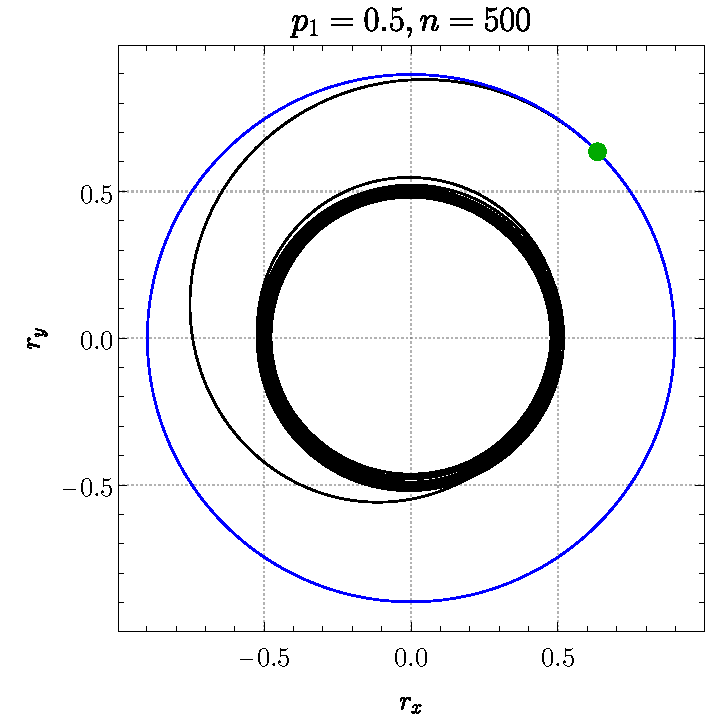
\includegraphics[width=1.\textwidth]{figures/maxent_results/local_all_ran_p=0.5_r=0.9_n=500_a=-3_b=3.pdf}
           \end{figure}
        \end{column}
    \end{columns}
\end{frame}
%###########################


%###########################
%########## AVG ############
\subsection{Compuertas de cómputo cuántico}
\begin{frame}{Compuerta SWAP}
    \begin{columns}
        \begin{column}{0.5\textwidth}
            Effective state before and after:
            \begin{align*}
                \rho(0)&=(1-p)\rho_{A}+p\rho_{B},\\
                \rho(t=1)&=p\rho_{A}+(1-p)\rho_{B}.
                \end{align*}
                Contraction!:
                \begin{equation*}
                    \kappa_{t}=\frac{r_{\rho(1)}}{r_{\rho(0)}}.
                  \end{equation*}
                  Non linear depolarizing channel:
                  \begin{equation*}
                      \boxed{\rho\mapsto\kappa_{1}^{\rho}\rho+(1-\kappa_{1}^{\rho})\frac{1}{2}\Id}
                    \end{equation*}
        \end{column}
        \begin{column}{0.5\textwidth}
            \begin{figure}[h!]
                \centering
                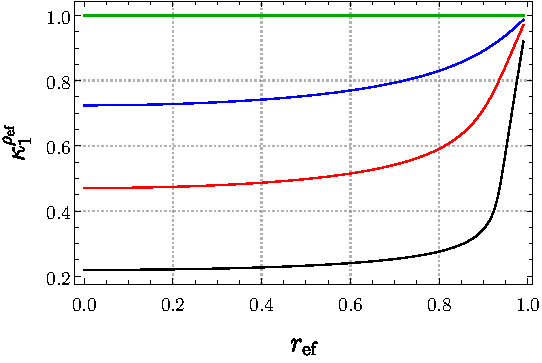
\includegraphics[width=0.9\linewidth]{figures/maxent_results/K(r).pdf}
                \caption{Depolarizing coefficient as a function of $r_{\rho(0)}$ for different values of $p$.}
                \label{fig:SWAPFactor2D}
              \end{figure}
        \end{column}
    \end{columns}
\end{frame}
\begin{frame}{Effective CNOT}
    We study
    \begin{equation*}
        \rho(t=1)=\CG{\cnot \mcA_{\mcC}^{max}[\rho(0)](\cnot)^{\dag}}
    \end{equation*}
    Initial efective state is
    \begin{equation*}
        \rho(0)=(1-p)\rho_{A}+p\rho_{B}.
    \end{equation*}
    Final efective state is
    \begin{align*}
        \rho(t=1)=&\frac{1}{2}[(1-p)(\rho(0)+\sigma_{3}\rho_{A}\sigma_{3}+\Tr{\sigma_{1}\rho_{B}}[\rho_{A}-\sigma_{3}\rho_{A}\sigma_{3}])\\
        &+p(\rho(0)+\sigma_{1}\rho_{B}\sigma_{1}+\Tr{\sigma_{3}\rho_{A}}[\rho_{B}-\sigma_{1}\rho_{B}\sigma_{1}])]
    \end{align*}.
\end{frame}
\begin{frame}{Phase flip channel}
    \begin{columns}
        \begin{column}{0.5\textwidth}
            Let's suppose $p=0$. The evolved effective state:
            \begin{equation*}
              \rho(t=1)=\frac{1}{2}\rho(0)+\frac{1}{2}\pauli{3}\rho(0)\pauli{3}.
            \end{equation*}
            This is a phase flip channel!
        \end{column}
        \begin{column}{0.5\textwidth}
            \begin{figure}[h!]
                \centering
                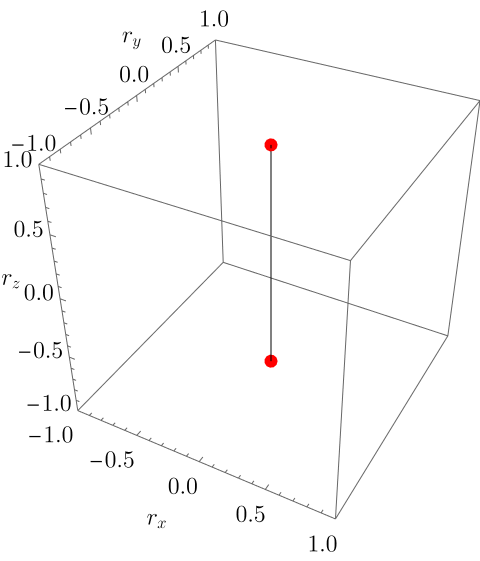
\includegraphics[width=0.7\linewidth]{figures/maxent_results/CNOT_p=1._t=1_r=0.9.png}
                \caption{Phase flip map}
                \label{fig:SWAPFactor2D}
              \end{figure}
        \end{column}
    \end{columns}
\end{frame}
\begin{frame}{Bit flip channel}
    \begin{columns}
        \begin{column}{0.5\textwidth}
            Let's suppose $p=1$. The evolved effective state:
            \begin{equation*}
              \rho(t=1)=\frac{1}{2}\rho(0)+\frac{1}{2}\pauli{1}\rho(0)\pauli{1}.
            \end{equation*}
        
            This is a bit flip channel!
        \end{column}
        \begin{column}{0.5\textwidth}
            \begin{figure}[h!]
                \centering
                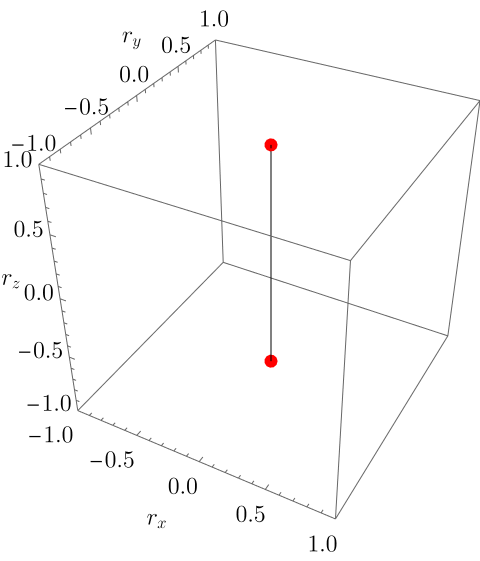
\includegraphics[width=0.7\linewidth]{figures/maxent_results/CNOT_p=1._t=1_r=0.9.png}
                \caption{Bit flip map}
                \label{fig:SWAPFactor2D}
              \end{figure}
        \end{column}
    \end{columns}
\end{frame}
\begin{frame}{Effective CNOT}
    Back to our expression:
    \begin{align*}
        \rho(t=1)=&\frac{1}{2}\rho(0)\\
        &+\frac{(1-p)}{2}\qty[\expval{\pauli{1}}_{\rho_{B}}\rho_{A}+(1-\expval{\pauli{1}}_{\rho_{B}})\pauli{3}\rho_{A}\pauli{3}]\\
        &+\frac{p}{2}\qty[\expval{\pauli{3}}_{\rho_{A}}\rho_{B}+(1-\expval{\pauli{3}}_{\rho_{A}})\pauli{1}\rho_{B}\pauli{1}].
    \end{align*}
    Mix of a non linear bit flip channel and a non linear phase flip channel
\end{frame}
\begin{frame}{Effective CNOT on the Bloch sphere}
    \begin{figure}[h!]
        \centering
        \begin{subfigure}{0.32\textwidth}
            \centering
            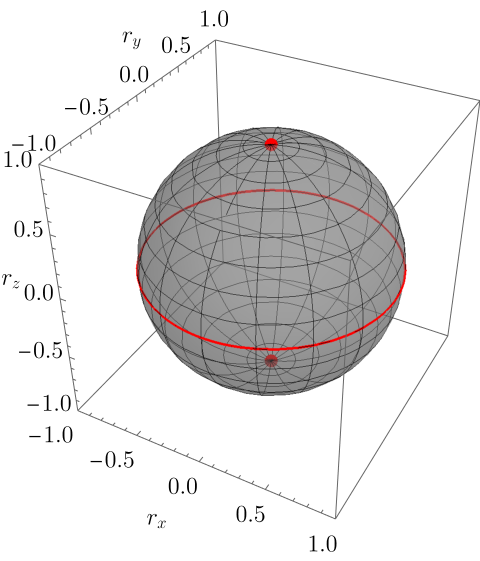
\includegraphics[width=0.9\linewidth]{figures/maxent_results/CNOT_p=0.5_t=0._r=0.9.png}
            \caption{$t=0.0$}
        \end{subfigure}%
        \begin{subfigure}{0.32\textwidth}
            \centering
            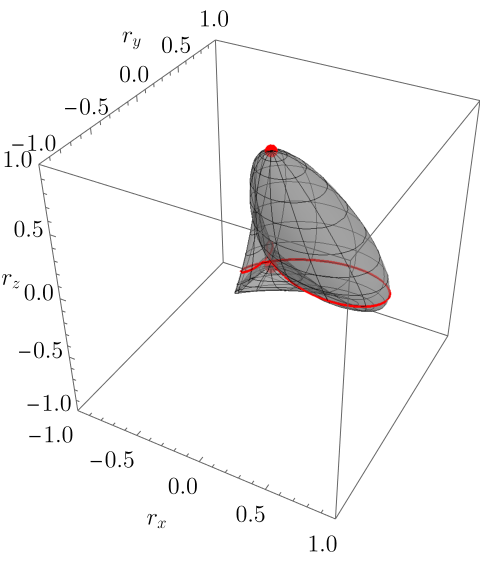
\includegraphics[width=0.9\linewidth]{figures/maxent_results/CNOT_p=0.5_t=1._r=0.9.png}
            \caption{$t=1.0$}
        \end{subfigure}
        \caption{Effect on the Bloch sphere. $r=0.8$, $p=0.4$.}
    \end{figure}
\end{frame}
%###########################


%###########################
%########## AVG ############
\subsection{Dinámicas especiales}

\begin{frame}{Canales de Pauli de N qubits}
    \begin{columns}
        \begin{column}{0.5\textwidth}
            El canal de Pauli sobre $n$ qubits más general está definido como
\begin{equation}\label{eq:PauliChannelN}
    \begin{gathered}
    P:\mcB(\hilbert_{2^{n}}) \rightarrow \mcB(\hilbert_{2^{n}})\nonumber\\
    P(\Delta)=\sum_{\vec{\alpha}}q_{\vec{\alpha}}\pauli{\vec{\alpha}}\Delta\pauli{\vec{\alpha}}, \,\text{ }\, \alpha_{k}\in\{0,1,2,3\} \rlap{.}
    \end{gathered}
\end{equation}
donde  $\pauli{\vec{\alpha}}=\pauli{\alpha_{1}}\otimes\pauli{\alpha_{2}}\otimes...\otimes \pauli{\alpha_{n}}$.
        \end{column}
        \begin{column}{0.5\textwidth}
            ¿O mejor primero poner el de dos?
        \end{column}
    \end{columns}
\end{frame}

\begin{frame}{Canales de dsfasamiento y despolarización}
    \begin{columns}
        \begin{column}{0.5\textwidth}
            Un ejemplo de tal $\mcE_{\pauli{j}}$ es el canal de Pauli
\begin{equation}
    \begin{gathered}
    P_{n,\pauli{j}}:\mcB(\hilbert_{2^{n}}) \rightarrow \mcB(\hilbert_{2^{n}})\nonumber\\
    P_{n,\pauli{j}}(\Delta)=\sum_{\vec{\alpha}}q_{\vec{\alpha}}\pauli{\vec{\alpha}}\Delta\pauli{\vec{\alpha}}, \,\text{ }\, \alpha_{k}\in\{0,j\} \nonumber\rlap{.}
    \end{gathered}
\end{equation}
Supóngase que se suma sobre todos los $2^{n}$ posibles vectores $\vec{\alpha}$, y con probabilidades $q_{\vec{\alpha}}=\frac{1-q_{\vec{0} }}{2^{n}-1}\,\forall\,\vec{\alpha}\neq\vec{0}$. Este es un canal de desfasamiento porque reduce la magnitud de los elementos fuera de la diagonal (en la base de los productos tensoriales de los eigenestados de $\pauli{j})$ por un factor de $\qty(1-\frac{2^{n}(1-q_{\vec{0}})}{2^{n}-1})$. Es sencillo ver que la dinámica efectiva corresponde al canal que reduce los elementos fuera de la diagonal (en la base de eigenestados de $\pauli{j}$) por el mismo factor.  Esto es, la dinámica efectiva es
\begin{align}
    \Gamma_{t}(\rho_{\ef})=&\qty(q_{\vec{0}}+\frac{2^{n-1}-1}{2^{n}-1}(1-q_{\vec{0}}))\rho_{\ef}\nonumber\\
    &+\qty(\frac{2^{n-1}}{2^{n}-1}(1-q_{\vec{0}}))\pauli{j}\rho_{\ef}\pauli{j}.\nonumber
\end{align}
        \end{column}
        \begin{column}{0.5\textwidth}
            El canal de despolarización es el canal cuántico que contrae de manera uniforme a todos los estados hacia el estado máximamente mezclado. Al canal de despolarización se le define como
\begin{gather}\label{eq:DepolarizingChannelN}
    D_{q}:\mcB(\hilbert_{2^{n}}) \rightarrow \mcB(\hilbert_{2^{n}})\nonumber\\
    D_{q}(\Delta)=q\Delta+(1-q)\Id_{2^{n}}\Tr(\Delta)\rlap{.}
\end{gather}
Para ver que el canal de despolarización es un canal de Pauli, véase que este puede reescribirse como 
\begin{equation}
    D_{q}(\varrho)=q\varrho+(1-q)\qty(P_{\pauli{1}}\circ P_{\pauli{3}})(\varrho).\nonumber
\end{equation}
La dinámica efectiva que corresponde al canal de despolarización no completo es simplemente
\begin{equation}
    \Gamma_{t}(\rho_{\ef})=q\rho_{\ef}+(1-q)\Id_{2}.\nonumber
\end{equation}
        \end{column}
    \end{columns}
\end{frame}

\begin{frame}{Canal de estabilización}
    \begin{columns}
        \begin{column}{0.5\textwidth}
            Considérese entonces que un sistema de $n$ partículas evoluciona siguiendo el canal cuántico
\begin{gather}
    \mcE_{\psi,t}:\mcB(\hilbert_{2^{n}}) \rightarrow \mcB(\hilbert_{2^{n}})\nonumber\\
    \mcE_{\psi,t}(\Delta)=e^{-t\mu}\varrho+(1-e^{-t \mu})\dyad{\psi}\Tr(\Delta)\rlap{.}\nonumber
\end{gather}
donde $\dyad{\psi}\in \densityspace{2^{n}}$
        \end{column}
        \begin{column}{0.5\textwidth}
            Ahora, sea $\rho_{\ef}$ un estado efectivo en $\densityspace{2}$ y $\varrho_{\max}$ el estado de máxima entropía en $\densityspace{2^{n}}$ compatible con este. Aplicando el modelo de grano grueso al estado de máxima entropía propagado por el canal de estabilización se obtiene que
\begin{equation}\label{eq:EffectiveStabilizing}
    \Gamma_{t}(\rho_{\ef})=e^{-t\mu}\rho(0)+(1-e^{-t \mu})\mcC(\dyad{\psi}).\nonumber
\end{equation}
Obsérvese que la dinámica efectiva es un canal cuántico, pero no necesariamente un canal de estabilización, pues el estado al que tiende el sistema efectivo, $\mcC(\dyad{\psi})$ no tiene por qué ser un estado puro. En realidad, en el caso en que $\ket{\psi}$ es un estado máximamente entrelazado, $\mcC(\dyad{\psi})$ es el estado máximamente mezclado, de tal manera que la dinámica efectiva es un canal de despolarización.
        \end{column}
    \end{columns}
\end{frame}
%###########################


%###########################
%########## AVG ############
\subsection{La asignación promedio}
\begin{frame}{Construcción de la asignación promedio}
    Otra forma de escoger un estado microscópico compatible es tomando un promedio\mycite{Macro-To-Micro}. Un promedio sobre el conjunto
    \begin{equation}
        \Omega_{\mcC}(\rho_{\ef}) = \{\ket{\psi}\in\hilbert_{m}:\, \mcC(\dyad{\psi}) = \rho_{\ef}  \}.\nonumber
    \end{equation}
    La aplicación de asignación promedio es el promedio sobre dicho conjunto, \ie 
    \begin{equation}
        \mcA_{\mcC}^{\avg}(\rho_{\ef}) =\int d \mu\,\, \delta(\mcC(\dyad{\psi})-\rho_{\ef})\,\dyad{\psi}.\nonumber
    \end{equation}
\end{frame}
\begin{frame}{Distancia entre la asignación promedio y la de máxima entropía}
    \begin{figure}
        \centering
        \begin{subfigure}{.45\textwidth}
          \centering
          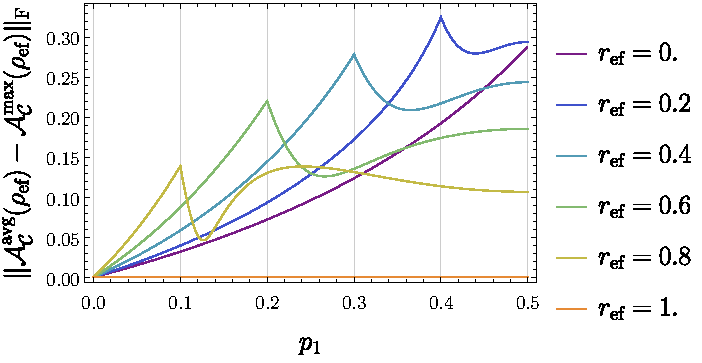
\includegraphics[width=1.\linewidth]{figures/avg_results/dist_maxent_avg_vs_p.pdf}
        \end{subfigure}%
        \begin{subfigure}{.45\textwidth}
          \centering
          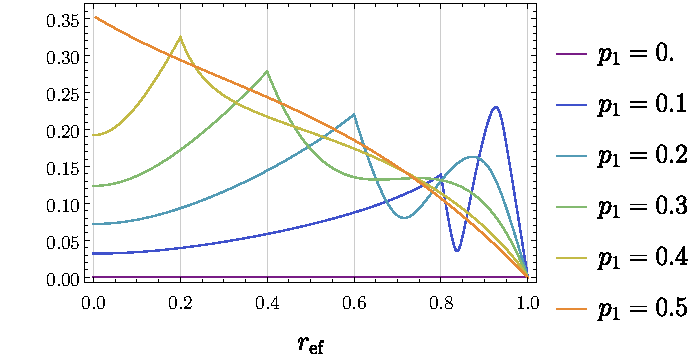
\includegraphics[width=1.\linewidth]{figures/avg_results/dist_maxent_avg_vs_z.pdf}
        \end{subfigure}
        \caption{Distancia de Frobenius entre asignaciones como función de $p_{1}$ para diferentes valores de $r_{z}$, y como función de $r_{z}$ para diferentes valores de $p_{1}$.}
    \end{figure}
\end{frame}
\begin{frame}{Discusión}
\begin{itemize}
    \item Iguales si el estado efectivo inicial es puro y si la aplicación de grano grueso se reduce a una traza parcial ($p_{1}\in\{0,1\}$).
    \item Notar que $\mcA_{\mcC}^{\max}(\Id_{2}/2)=\Id_{4}/4$ mientras que $\mcA_{\mcC}^{\avg}(\Id_{2}/2)\neq\Id_{4}/4$.
\end{itemize}
\end{frame}
%###########################
